\documentclass[aspectratio=169, 11pt]{beamer}

% ── Theme & Colors ──────────────────────────────────────────────
\usetheme{default}
\usecolortheme{default}
\setbeamertemplate{navigation symbols}{}
\setbeamertemplate{footline}[frame number]
\setbeamertemplate{itemize items}[circle]

% ── Packages ────────────────────────────────────────────────────
\usepackage[T1]{fontenc}
\usepackage{lmodern}
\usepackage{graphicx}
\usepackage{booktabs}
\usepackage{tikz}
\usepackage{pgfplots}
\pgfplotsset{compat=1.18}
\usetikzlibrary{arrows.meta, positioning, shapes.geometric, calc, backgrounds, fit, decorations.pathreplacing}
\usepackage{xcolor}
\usepackage{fontawesome5}
\usepackage{adjustbox}
\usepackage{multicol}
\usepackage{amsmath}

% ── Color Palette ───────────────────────────────────────────────
\definecolor{primary}{HTML}{1A1A2E}
\definecolor{accent}{HTML}{E94560}
\definecolor{accentblue}{HTML}{0F3460}
\definecolor{softgray}{HTML}{F5F5F5}
\definecolor{darktext}{HTML}{2C2C2C}
\definecolor{graphgreen}{HTML}{2ECC71}
\definecolor{densepurple}{HTML}{9B59B6}
\definecolor{tfidfblue}{HTML}{3498DB}
\definecolor{hybridorange}{HTML}{E67E22}
\definecolor{lightaccent}{HTML}{FDE8EC}
\definecolor{lightgreen}{HTML}{E8F8F0}
\definecolor{lightblue}{HTML}{EBF5FB}
\definecolor{lightorange}{HTML}{FEF5E7}
\definecolor{dimgray}{HTML}{95A5A6}
\definecolor{softpurple}{HTML}{EDE9FE}

% ── Beamer Styling ──────────────────────────────────────────────
\setbeamercolor{structure}{fg=primary}
\setbeamercolor{title}{fg=white}
\setbeamercolor{frametitle}{fg=primary}
\setbeamercolor{normal text}{fg=darktext}
\setbeamercolor{itemize item}{fg=accent}
\setbeamercolor{itemize subitem}{fg=accentblue}
\setbeamerfont{frametitle}{size=\Large, series=\bfseries}
\setbeamerfont{title}{size=\huge, series=\bfseries}

% ── Custom macros ───────────────────────────────────────────────
\newcommand{\sectionslide}[2]{%
  \begin{frame}[plain]
    \begin{tikzpicture}[remember picture, overlay]
      \fill[primary] (current page.south west) rectangle (current page.north east);
      \node[anchor=center, text=white, font=\Huge\bfseries] at ([yshift=0.5cm]current page.center) {#1};
      \node[anchor=center, text=accent, font=\large] at ([yshift=-0.8cm]current page.center) {#2};
    \end{tikzpicture}
  \end{frame}
}
\newcommand{\metricbox}[3]{%
  \begin{tikzpicture}
    \node[rounded corners=5pt, fill=#1!10, draw=#1, line width=0.6pt,
          minimum width=2.8cm, minimum height=1.5cm, align=center] {
      {\color{#1}\large\bfseries #2}\\[2pt]
      {\small #3}
    };
  \end{tikzpicture}
}

\title{GraphRAG for Domain-Specific LLMs}
\subtitle{Knowledge-Graph Retrieval over Supply-Chain Reports}
\author{Jaafar Yeffou}
\date{2025\,--\,2026}
\institute{Generative AI Course --- University Final Project}

% ════════════════════════════════════════════════════════════════
\begin{document}

% ── Slide 1: Title ──────────────────────────────────────────────
{
\setbeamertemplate{footline}{}
\begin{frame}[plain]
  \begin{tikzpicture}[remember picture, overlay]
    \fill[primary] (current page.south west) rectangle (current page.north east);
    \fill[accent, opacity=0.15] ([xshift=-3cm, yshift=-2cm]current page.north east) circle (5cm);
    \fill[accentblue, opacity=0.2] ([xshift=2cm, yshift=1cm]current page.south west) circle (4cm);
    \node[anchor=center, text=white, font=\Huge\bfseries, text width=12cm, align=center]
      at ([yshift=1.8cm]current page.center)
      {GraphRAG for\\Domain-Specific LLMs};
    \node[anchor=center, text=accent, font=\large, text width=12cm, align=center]
      at ([yshift=0.2cm]current page.center)
      {Knowledge-Graph Retrieval\\over Supply-Chain Reports};
    \draw[accent, line width=1pt] ([xshift=-3cm, yshift=-0.6cm]current page.center)
      -- ([xshift=3cm, yshift=-0.6cm]current page.center);
    \node[anchor=center, text=white!80, font=\Large]
      at ([yshift=-1.4cm]current page.center)
      {Jaafar Yeffou};
    \node[anchor=center, text=white!50, font=\small]
      at ([yshift=-2.4cm]current page.center)
      {Generative AI --- University Final Project --- 2025/2026};
  \end{tikzpicture}
\end{frame}
}

% ── Slide 2: The Core Idea ──────────────────────────────────────
\begin{frame}{The Core Idea}
  \centering
  \vspace{6pt}
  \begin{tikzpicture}
    % LEFT: traditional search
    \node[draw=dimgray, rounded corners=8pt, fill=softgray, text width=5cm, align=center,
          minimum height=3.2cm, inner sep=10pt] (trad) at (-4,0) {
      {\color{dimgray}\Large\faIcon{search}}\\[6pt]
      {\large\bfseries\color{dimgray} Traditional Search}\\[8pt]
      {\small\color{dimgray}
        Finds pages that contain\\
        the \textbf{same words}\\
        as your question.\\[4pt]
        \textit{``Where did I see this word?''}
      }
    };
    % RIGHT: GraphRAG
    \node[draw=graphgreen, rounded corners=8pt, fill=lightgreen, text width=5cm, align=center,
          minimum height=3.2cm, inner sep=10pt, line width=1.2pt] (graph) at (4,0) {
      {\color{graphgreen}\Large\faIcon{project-diagram}}\\[6pt]
      {\large\bfseries\color{graphgreen} GraphRAG}\\[8pt]
      {\small\color{darktext}
        Builds a \textbf{map of connections}\\
        between concepts, then navigates\\
        that map to find evidence.\\[4pt]
        \textit{``How are these ideas connected?''}
      }
    };
    % VS
    \node[circle, draw=accent, fill=lightaccent, minimum size=1cm,
          font=\bfseries\color{accent}] at (0,0) {vs};
    % Bottom takeaway
    \node[draw=accent, rounded corners=6pt, fill=lightaccent, text width=11cm, align=center, inner sep=8pt]
      at (0,-2.8) {
      {\small\color{darktext}
        \textbf{Question:} ``How does diversification strengthen resilience?''\\[2pt]
        Traditional search looks for pages with those words.
        \textbf{\color{graphgreen}GraphRAG} follows the connection\\
        \textbf{\color{graphgreen}Diversification}
        $\xrightarrow{\text{\footnotesize\color{accent}STRENGTHENS}}$
        \textbf{\color{graphgreen}Resilience} and returns the \textit{evidence behind the link}.}
    };
  \end{tikzpicture}
\end{frame}

% ── Slide 3: From PDFs to Chunks ────────────────────────────────
\begin{frame}{From PDFs to Chunks}
  \centering
  \vspace{4pt}
  \begin{tikzpicture}[
    node distance=0.45cm and 0.8cm,
    box/.style={draw=accentblue, rounded corners=6pt, fill=lightblue,
                 minimum width=2.6cm, minimum height=1.5cm, align=center, font=\small},
    arr/.style={-{Stealth[length=6pt]}, thick, accent},
  ]
    % Step 1
    \node[box] (pdf) {\faIcon{file-pdf}\\[2pt]\textbf{10 Real PDFs}\\[-1pt]{\tiny OECD, WTO,}\\[-2pt]{\tiny World Bank, UNCTAD}};
    % Step 2
    \node[box, right=of pdf] (pages) {\faIcon{file-alt}\\[2pt]\textbf{Page Extraction}\\[-1pt]{\tiny Each page's text}\\[-2pt]{\tiny is read separately}};
    % Step 3
    \node[box, right=of pages] (chunks) {\faIcon{puzzle-piece}\\[2pt]\textbf{2{,}022 Chunks}\\[-1pt]{\tiny 1{,}000 chars each}\\[-2pt]{\tiny 150 char overlap}};
    % Step 4
    \node[draw=graphgreen, rounded corners=6pt, fill=lightgreen, line width=1.2pt,
          minimum width=2.6cm, minimum height=1.5cm, align=center, font=\small,
          right=of chunks] (graphstep) {{\color{graphgreen}\faIcon{project-diagram}}\\[2pt]\textbf{\color{graphgreen}Graph Build}\\[-1pt]{\tiny\color{darktext} Entities \& relations}\\[-2pt]{\tiny\color{darktext} extracted per chunk}};

    \draw[arr] (pdf) -- (pages);
    \draw[arr] (pages) -- (chunks);
    \draw[arr] (chunks) -- (graphstep);
  \end{tikzpicture}

  \vspace{12pt}
  \begin{columns}[T]
    \begin{column}{0.48\textwidth}
      \centering
      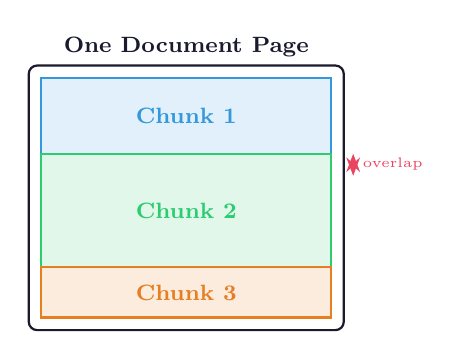
\begin{tikzpicture}[scale=0.8]
        \draw[thick, primary, rounded corners=3pt] (0,0) rectangle (5,4.2);
        \node[font=\footnotesize\bfseries, primary] at (2.5,4.5) {One Document Page};
        \fill[tfidfblue!15] (0.2,2.8) rectangle (4.8,4);
        \draw[tfidfblue, thick] (0.2,2.8) rectangle (4.8,4);
        \node[font=\footnotesize\bfseries, tfidfblue] at (2.5,3.4) {Chunk 1};
        \fill[accent!15] (0.2,2.45) rectangle (4.8,2.8);
        \fill[graphgreen!15] (0.2,1.0) rectangle (4.8,2.8);
        \draw[graphgreen, thick] (0.2,1.0) rectangle (4.8,2.8);
        \node[font=\footnotesize\bfseries, graphgreen] at (2.5,1.9) {Chunk 2};
        \fill[accent!15] (0.2,0.65) rectangle (4.8,1.0);
        \fill[hybridorange!15] (0.2,0.2) rectangle (4.8,1.0);
        \draw[hybridorange, thick] (0.2,0.2) rectangle (4.8,1.0);
        \node[font=\footnotesize\bfseries, hybridorange] at (2.5,0.6) {Chunk 3};
        % overlap labels
        \draw[{Stealth}-{Stealth}, accent, thick] (5.15,2.45) -- (5.15,2.8);
        \node[font=\tiny, accent, right] at (5.15,2.63) {overlap};
      \end{tikzpicture}
    \end{column}
    \begin{column}{0.48\textwidth}
      \textbf{\color{accent}Why chunk with overlap?}\\[6pt]
      {\small
        An important sentence may sit at the\\
        boundary between two sections.\\[4pt]
        The \textbf{150-character overlap} ensures both\\
        neighboring chunks carry that context.\\[4pt]
        Each chunk gets a \textbf{unique ID}:\\
        {\color{accentblue}\texttt{doc\_id:page:chunk\_index}}\\
        so every piece of evidence is traceable.
      }
    \end{column}
  \end{columns}
\end{frame}

% ── Slide 4: What Makes GraphRAG Different ──────────────────────
\begin{frame}{What Makes GraphRAG Different}
  \centering
  \vspace{4pt}
  \begin{tikzpicture}
    % Three steps visual
    % Step A: Read
    \node[draw=accentblue, rounded corners=8pt, fill=lightblue,
          text width=3.5cm, align=center, minimum height=2.5cm, inner sep=8pt]
      (stepA) at (-5,0) {
      {\color{accentblue}\Large\faIcon{book-open}}\\[4pt]
      {\bfseries\color{accentblue} 1. Read Each Chunk}\\[6pt]
      {\small\color{darktext}
        Split every chunk\\
        into sentences and\\
        scan for known\\
        domain concepts.
      }
    };
    % Step B: Connect
    \node[draw=graphgreen, rounded corners=8pt, fill=lightgreen, line width=1.2pt,
          text width=3.5cm, align=center, minimum height=2.5cm, inner sep=8pt]
      (stepB) at (0,0) {
      {\color{graphgreen}\Large\faIcon{project-diagram}}\\[4pt]
      {\bfseries\color{graphgreen} 2. Build the Map}\\[6pt]
      {\small\color{darktext}
        Draw arrows between\\
        concepts based on\\
        what the sentence\\
        actually says.
      }
    };
    % Step C: Navigate
    \node[draw=accent, rounded corners=8pt, fill=lightaccent,
          text width=3.5cm, align=center, minimum height=2.5cm, inner sep=8pt]
      (stepC) at (5,0) {
      {\color{accent}\Large\faIcon{route}}\\[4pt]
      {\bfseries\color{accent} 3. Navigate to Answer}\\[6pt]
      {\small\color{darktext}
        When you ask a question,\\
        follow the arrows that\\
        match what you're\\
        asking about.
      }
    };
    \draw[-{Stealth[length=6pt]}, thick, primary] (stepA) -- (stepB);
    \draw[-{Stealth[length=6pt]}, thick, primary] (stepB) -- (stepC);

    % Bottom insight
    \node[draw=graphgreen, rounded corners=6pt, fill=lightgreen, text width=12cm,
          align=center, inner sep=8pt] at (0,-2.6) {
      {\small\color{darktext}
        Think of it like a \textbf{subway map} of supply-chain knowledge.\\
        Entities are stations. Relations are the lines between them.\\
        GraphRAG finds the \textbf{route} that answers your question.
      }
    };
  \end{tikzpicture}
\end{frame}

% ── Slide 5: The Domain Schema ──────────────────────────────────
\begin{frame}{The Domain Schema --- What the Graph Knows}
  \begin{columns}[T]
    \begin{column}{0.48\textwidth}
      \textbf{\color{accent}8 Entity Types}\\[4pt]
      {\small Each type has a \textbf{weight} reflecting how informative it is:}\\[6pt]
      \begin{tikzpicture}[
        label/.style={font=\footnotesize, anchor=east},
      ]
        \foreach \etype/\w/\col/\ypos in {
          strategy/3.0/accent/3.2,
          policy/2.9/accent/2.7,
          capability/2.6/accentblue/2.2,
          risk/2.4/accentblue/1.7,
          actor/1.9/densepurple/1.2,
          sector/1.9/densepurple/0.7,
          system/1.1/dimgray/0.2,
          organization/0.7/dimgray/-0.3%
        } {
          \fill[\col!20, rounded corners=2pt] (0,\ypos-0.12) rectangle (\w*1.4,\ypos+0.12);
          \draw[\col!50, rounded corners=2pt] (0,\ypos-0.12) rectangle (\w*1.4,\ypos+0.12);
          \node[label] at (-0.1,\ypos) {\etype};
          \node[font=\tiny\bfseries, text=\col] at (\w*1.4+0.35,\ypos) {\w};
        }
        \node[font=\tiny\itshape, dimgray] at (2,-0.8) {\faIcon{info-circle}~Higher weight = more informative};
      \end{tikzpicture}
    \end{column}
    \begin{column}{0.48\textwidth}
      \textbf{\color{accentblue}Concrete Examples}\\[6pt]
      {\small
        \textbf{\color{accent}strategy:} Diversification, Reshoring,\\
        \hspace*{1.2cm}Nearshoring, Just-in-Time\\[3pt]
        \textbf{\color{accent}policy:} Trade Facilitation,\\
        \hspace*{1.2cm}Export Restrictions\\[3pt]
        \textbf{\color{accentblue}capability:} Resilience, Flexibility,\\
        \hspace*{1.2cm}Visibility, Agility\\[3pt]
        \textbf{\color{accentblue}risk:} COVID-19, Bottleneck,\\
        \hspace*{1.2cm}Concentration, Shortage\\[3pt]
        \textbf{\color{densepurple}sector:} Semiconductors, Food,\\
        \hspace*{1.2cm}Pharmaceuticals\\[6pt]
      }
      \textbf{\color{graphgreen}Intuition:}\\
      {\small A \textit{strategy} appearing in a chunk\\
      tells us much more than an \textit{organization}\\
      name appearing --- the weights capture this.}
    \end{column}
  \end{columns}
\end{frame}

% ── Slide 6: Entity Extraction --- The Reading Step ─────────────
\begin{frame}{Entity Extraction --- The Reading Step}
  \centering
  \vspace{2pt}
  % Input sentence
  \begin{tikzpicture}
    \node[draw=accentblue, rounded corners=6pt, fill=lightblue, text width=13cm,
          align=left, inner sep=10pt] (sent) {
      {\footnotesize\color{dimgray}\faIcon{file-alt}~Sentence from a chunk:}\\[4pt]
      {\normalsize ``\textbf{\color{accent}Diversification} of suppliers
      \textbf{\color{accentblue}strengthens} \textbf{\color{graphgreen}resilience}
      against \textbf{\color{hybridorange}supply chain disruptions}.''}
    };
  \end{tikzpicture}

  \vspace{6pt}
  \begin{tikzpicture}[
    card/.style={draw=##1, rounded corners=6pt, fill=##1!8,
                  text width=3.8cm, align=center, inner sep=8pt, minimum height=2.5cm},
    arr/.style={-{Stealth[length=5pt]}, thick, accent},
  ]
    % Step 1
    \node[card=accent] (s1) at (-4.5,0) {
      {\color{accent}\bfseries\faIcon{tags}~Recognize Entities}\\[6pt]
      {\footnotesize\color{darktext}
        Each word is matched against\\
        a vocabulary of known aliases:\\[3pt]
        ``diversification'' $\to$\\
        \textbf{\color{accent}Diversification} {\tiny(strategy)}\\[2pt]
        ``resilience'' $\to$\\
        \textbf{\color{graphgreen}Resilience} {\tiny(capability)}\\[2pt]
        ``supply chain disruptions'' $\to$\\
        \textbf{\color{hybridorange}SC Disruption} {\tiny(risk)}
      }
    };
    % Step 2
    \node[card=accentblue] (s2) at (0,0) {
      {\color{accentblue}\bfseries\faIcon{bolt}~Detect the Verb}\\[6pt]
      {\footnotesize\color{darktext}
        The system looks for\\
        \textbf{trigger words} that\\
        signal a relationship:\\[4pt]
        ``strengthens'' $\to$\\
        means \textbf{\color{accentblue}STRENGTHENS}\\[4pt]
        ``reduces'' $\to$ MITIGATES\\
        ``exposes'' $\to$ EXPOSES\\
        ``trade-off'' $\to$ TRADE\_OFF\\
      }
    };
    % Step 3
    \node[card=graphgreen] (s3) at (4.5,0) {
      {\color{graphgreen}\bfseries\faIcon{project-diagram}~Create the Link}\\[6pt]
      {\footnotesize\color{darktext}
        An arrow is drawn\\
        in the knowledge graph:\\[6pt]
        {\color{accent}Diversification}\\
        {\color{accentblue}$\longrightarrow$\,\textsc{\tiny strengthens}}\\
        {\color{graphgreen}Resilience}\\[6pt]
        With the original sentence\\
        kept as \textbf{evidence}.
      }
    };
    \draw[arr] (s1) -- (s2);
    \draw[arr] (s2) -- (s3);
  \end{tikzpicture}
\end{frame}

% ── Slide 7: Relation Types ────────────────────────────────────
\begin{frame}{7 Relation Types --- The Arrows on the Map}
  \centering
  \vspace{2pt}
  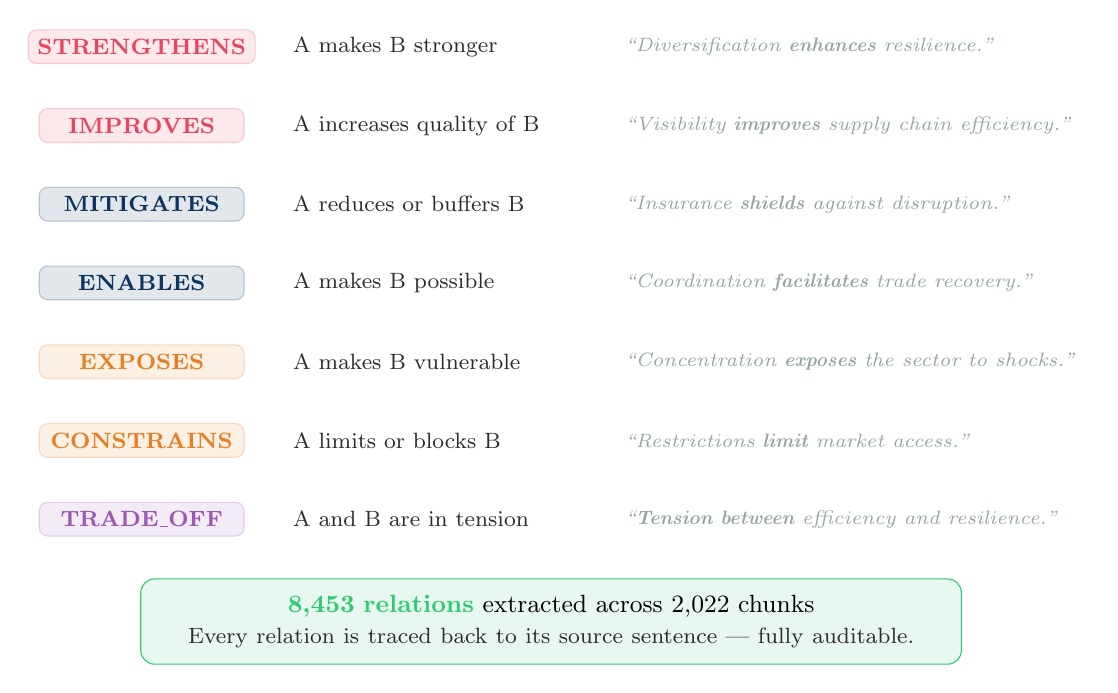
\begin{tikzpicture}
    % Row helper: \relrow{y}{color}{LABEL}{meaning}{example}
    % STRENGTHENS
    \node[rounded corners=3pt, fill=accent!12, draw=accent!30, font=\footnotesize\bfseries,
          text=accent, minimum width=2.6cm, align=center] at (-5.2,4.5) {STRENGTHENS};
    \node[font=\footnotesize, text=darktext, anchor=west, text width=3.6cm] at (-3.4,4.5) {A makes B stronger};
    \node[font=\scriptsize\itshape, text=dimgray, anchor=west, text width=5.8cm] at (0.8,4.5) {``Diversification \textbf{enhances} resilience.''};
    % IMPROVES
    \node[rounded corners=3pt, fill=accent!12, draw=accent!30, font=\footnotesize\bfseries,
          text=accent, minimum width=2.6cm, align=center] at (-5.2,3.5) {IMPROVES};
    \node[font=\footnotesize, text=darktext, anchor=west, text width=3.6cm] at (-3.4,3.5) {A increases quality of B};
    \node[font=\scriptsize\itshape, text=dimgray, anchor=west, text width=5.8cm] at (0.8,3.5) {``Visibility \textbf{improves} supply chain efficiency.''};
    % MITIGATES
    \node[rounded corners=3pt, fill=accentblue!12, draw=accentblue!30, font=\footnotesize\bfseries,
          text=accentblue, minimum width=2.6cm, align=center] at (-5.2,2.5) {MITIGATES};
    \node[font=\footnotesize, text=darktext, anchor=west, text width=3.6cm] at (-3.4,2.5) {A reduces or buffers B};
    \node[font=\scriptsize\itshape, text=dimgray, anchor=west, text width=5.8cm] at (0.8,2.5) {``Insurance \textbf{shields} against disruption.''};
    % ENABLES
    \node[rounded corners=3pt, fill=accentblue!12, draw=accentblue!30, font=\footnotesize\bfseries,
          text=accentblue, minimum width=2.6cm, align=center] at (-5.2,1.5) {ENABLES};
    \node[font=\footnotesize, text=darktext, anchor=west, text width=3.6cm] at (-3.4,1.5) {A makes B possible};
    \node[font=\scriptsize\itshape, text=dimgray, anchor=west, text width=5.8cm] at (0.8,1.5) {``Coordination \textbf{facilitates} trade recovery.''};
    % EXPOSES
    \node[rounded corners=3pt, fill=hybridorange!12, draw=hybridorange!30, font=\footnotesize\bfseries,
          text=hybridorange, minimum width=2.6cm, align=center] at (-5.2,0.5) {EXPOSES};
    \node[font=\footnotesize, text=darktext, anchor=west, text width=3.6cm] at (-3.4,0.5) {A makes B vulnerable};
    \node[font=\scriptsize\itshape, text=dimgray, anchor=west, text width=5.8cm] at (0.8,0.5) {``Concentration \textbf{exposes} the sector to shocks.''};
    % CONSTRAINS
    \node[rounded corners=3pt, fill=hybridorange!12, draw=hybridorange!30, font=\footnotesize\bfseries,
          text=hybridorange, minimum width=2.6cm, align=center] at (-5.2,-0.5) {CONSTRAINS};
    \node[font=\footnotesize, text=darktext, anchor=west, text width=3.6cm] at (-3.4,-0.5) {A limits or blocks B};
    \node[font=\scriptsize\itshape, text=dimgray, anchor=west, text width=5.8cm] at (0.8,-0.5) {``Restrictions \textbf{limit} market access.''};
    % TRADE_OFF
    \node[rounded corners=3pt, fill=densepurple!12, draw=densepurple!30, font=\footnotesize\bfseries,
          text=densepurple, minimum width=2.6cm, align=center] at (-5.2,-1.5) {TRADE\_OFF};
    \node[font=\footnotesize, text=darktext, anchor=west, text width=3.6cm] at (-3.4,-1.5) {A and B are in tension};
    \node[font=\scriptsize\itshape, text=dimgray, anchor=west, text width=5.8cm] at (0.8,-1.5) {``\textbf{Tension between} efficiency and resilience.''};
    % Bottom note
    \node[draw=graphgreen, rounded corners=5pt, fill=lightgreen,
          text width=10cm, align=center, inner sep=6pt, font=\small]
      at (0,-2.8) {
      \textbf{\color{graphgreen}8{,}453 relations} extracted across 2{,}022 chunks\\
      {\footnotesize\color{darktext} Every relation is traced back to its source sentence --- fully auditable.}
    };
  \end{tikzpicture}
\end{frame}

% ── Slide 8: The Knowledge Graph ────────────────────────────────
\begin{frame}{The Knowledge Graph in Action}
  \centering
  \begin{tikzpicture}[scale=0.82, transform shape,
    entity/.style={circle, draw=##1, fill=##1!15, minimum size=1.3cm, font=\tiny\bfseries, align=center, text=darktext},
    entitybig/.style={circle, draw=##1, fill=##1!20, minimum size=1.6cm, font=\scriptsize\bfseries, align=center, text=darktext, line width=1.2pt},
    chunk/.style={rectangle, draw=accentblue!40, fill=lightblue, rounded corners=3pt, minimum width=1.6cm, minimum height=0.55cm, font=\tiny, align=center, text=darktext},
    rel/.style={-{Stealth[length=4pt]}, thick, ##1},
  ]
    % Entity nodes
    \node[entitybig=accent]     (div)   at (0,3.5)    {Diversi-\\fication};
    \node[entitybig=graphgreen] (res)   at (5,4)      {Resilience};
    \node[entitybig=accentblue] (eff)   at (10,3.5)   {Efficiency};
    \node[entity=hybridorange]  (covid) at (2,6)      {COVID-19};
    \node[entity=densepurple]   (jit)   at (7.5,6)    {Just-in-\\Time};
    \node[entity=tfidfblue]     (vis)   at (12,5.5)   {Visibility};
    \node[entity=accent]        (nsh)   at (-2.5,5.5) {Near-\\shoring};

    % Relation edges
    \draw[rel=graphgreen, line width=1.5pt] (div) -- node[above, font=\tiny\bfseries, text=graphgreen] {STRENGTHENS} (res);
    \draw[rel=hybridorange] (res) -- node[above, font=\tiny\bfseries, text=hybridorange] {TRADE\_OFF} (eff);
    \draw[rel=accentblue] (jit) -- node[right, font=\tiny\bfseries, text=accentblue, pos=0.4] {IMPROVES} (eff);
    \draw[rel=hybridorange] (covid) -- node[left, font=\tiny\bfseries, text=hybridorange, pos=0.4] {AFFECTS} (div);
    \draw[rel=densepurple] (covid) -- node[above, font=\tiny\bfseries, text=densepurple] {EXPOSES} (jit);
    \draw[rel=tfidfblue] (vis) -- node[right, font=\tiny\bfseries, text=tfidfblue, pos=0.4] {ENABLES} (res);
    \draw[rel=accent] (nsh) -- node[left, font=\tiny\bfseries, text=accent, pos=0.4] {MITIGATES} (covid);

    % Chunk nodes below
    \node[chunk] (c1) at (0,1)  {Chunk p12:c02};
    \node[chunk] (c2) at (5,1)  {Chunk p45:c01};
    \node[chunk] (c3) at (10,1) {Chunk p78:c00};

    % MENTIONED_IN dashed edges
    \draw[dashed, dimgray!50] (div) -- (c1);
    \draw[dashed, dimgray!50] (div) -- (c2);
    \draw[dashed, dimgray!50] (res) -- (c2);
    \draw[dashed, dimgray!50] (res) -- (c3);
    \draw[dashed, dimgray!50] (eff) -- (c3);

    % Stats box
    \node[draw=graphgreen, rounded corners=5pt, fill=lightgreen, font=\small, align=center, inner sep=6pt]
      at (5,-0.8) {
      \textbf{\color{graphgreen}258} entities \quad
      \textbf{\color{graphgreen}8{,}453} relations \quad
      \textbf{\color{graphgreen}14{,}889} sentences \quad
      \textbf{\color{graphgreen}16{,}658} mention links
    };
  \end{tikzpicture}
\end{frame}

% ── Slide 9: Query Intent Detection ────────────────────────────
\begin{frame}{Understanding the Question Before Searching}
  \centering
  \vspace{4pt}
  {\small Before retrieving anything, GraphRAG reads the question and asks: \textbf{\color{accent}what kind of answer is this looking for?}}\\[10pt]
  \begin{tikzpicture}[
    qcard/.style={draw=##1, rounded corners=6pt, fill=##1!8, text width=3.6cm,
                   align=center, inner sep=8pt, minimum height=2.8cm},
  ]
    \node[qcard=graphgreen] (q1) at (-4.8,0) {
      {\color{graphgreen}\bfseries\faIcon{arrow-right}~Causal}\\[6pt]
      {\footnotesize ``\textbf{How does} X \textbf{improve} Y?''}\\[6pt]
      {\scriptsize\color{darktext}
        Looks for arrows like:\\
        STRENGTHENS, MITIGATES,\\
        ENABLES
      }
    };
    \node[qcard=hybridorange] (q2) at (0,0) {
      {\color{hybridorange}\bfseries\faIcon{exchange-alt}~Trade-off}\\[6pt]
      {\footnotesize ``What is the \textbf{trade-off}\\between X and Y?''}\\[6pt]
      {\scriptsize\color{darktext}
        Looks for arrows like:\\
        TRADE\_OFF\_WITH,\\
        CONSTRAINS
      }
    };
    \node[qcard=accentblue] (q3) at (4.8,0) {
      {\color{accentblue}\bfseries\faIcon{question-circle}~Explanation}\\[6pt]
      {\footnotesize ``\textbf{Why} are supply chains\\vulnerable to shocks?''}\\[6pt]
      {\scriptsize\color{darktext}
        Looks for arrows like:\\
        EXPOSES, AFFECTS,\\
        CONSTRAINS
      }
    };

    % Bottom result
    \node[draw=accent, rounded corners=6pt, fill=lightaccent, text width=12cm,
          align=center, inner sep=8pt] at (0,-2.6) {
      {\small\color{darktext}
        \textbf{\color{accent}This is key:} if you ask a causal question and a chunk has a\\
        \textbf{STRENGTHENS} relation between your two concepts, that chunk gets a \textbf{big bonus}.\\
        If it only has TRADE\_OFF (wrong intent), it gets \textbf{penalized}.
      }
    };
  \end{tikzpicture}
\end{frame}

% ── Slide 10: Entity Specificity ────────────────────────────────
\begin{frame}{Not All Entities Are Equal}
  \centering
  \vspace{4pt}
  {\small The system gives more weight to \textbf{rare, specific} concepts and penalizes generic ones.}\\[10pt]
  \begin{tikzpicture}
    % High specificity side
    \node[draw=graphgreen, rounded corners=8pt, fill=lightgreen, text width=5.5cm,
          align=center, inner sep=10pt, minimum height=3.5cm] (high) at (-3.8,0) {
      {\color{graphgreen}\large\bfseries\faIcon{star}~High Specificity}\\[8pt]
      {\small\color{darktext}
        \textbf{Nearshoring} (strategy)\\
        appears in only 5 out of 2{,}022 chunks\\[4pt]
        $\to$ \textbf{Very strong signal:}\\
        if a chunk mentions nearshoring,\\
        it's probably about nearshoring.
      }
    };
    % Low specificity side
    \node[draw=hybridorange, rounded corners=8pt, fill=lightorange, text width=5.5cm,
          align=center, inner sep=10pt, minimum height=3.5cm] (low) at (3.8,0) {
      {\color{hybridorange}\large\bfseries\faIcon{globe}~Low Specificity}\\[8pt]
      {\small\color{darktext}
        \textbf{Supply Chain} (system)\\
        appears in 90\% of all chunks\\[4pt]
        $\to$ \textbf{Almost worthless:}\\
        every chunk mentions it,\\
        so it doesn't help distinguish.
      }
    };

    % Formula underneath
    \node[draw=accentblue, rounded corners=6pt, fill=lightblue, text width=12cm,
          align=center, inner sep=8pt] at (0,-2.8) {
      {\small\color{darktext}
        \textbf{\color{accentblue}Specificity} $=$ $\dfrac{\text{entity type weight}}{\log(1 + \text{how many chunks mention it})}$
        \quad---\quad entities that appear everywhere are automatically downweighted.
      }
    };
  \end{tikzpicture}
\end{frame}

% ── Slide 11: Graph Scoring ─────────────────────────────────────
\begin{frame}{How GraphRAG Scores Every Chunk}
  \centering
  \vspace{2pt}
  {\small For each chunk, the system computes a score from \textbf{\color{graphgreen}6 positive signals} and \textbf{\color{accent}3 penalties}:}\\[8pt]
  \begin{tikzpicture}[
    pos/.style={draw=graphgreen!40, rounded corners=5pt, fill=lightgreen,
                text width=3.6cm, align=center, inner sep=6pt, minimum height=1.1cm},
    neg/.style={draw=accent!40, rounded corners=5pt, fill=lightaccent,
                text width=3.6cm, align=center, inner sep=6pt, minimum height=1.1cm},
  ]
    % Positive row 1
    \node[pos] (em) at (-4.8,2) {
      {\color{graphgreen}\scriptsize\bfseries Entity Match}\\
      {\tiny\color{darktext} Are query concepts in this chunk?}
    };
    \node[pos] (cb) at (0,2) {
      {\color{graphgreen}\scriptsize\bfseries Coverage Bonus}\\
      {\tiny\color{darktext} How many query concepts appear together?}
    };
    \node[pos] (sa) at (4.8,2) {
      {\color{graphgreen}\scriptsize\bfseries Sentence Alignment}\\
      {\tiny\color{darktext} Do concepts co-occur in same sentences?}
    };
    % Positive row 2
    \node[pos] (dr) at (-4.8,0.5) {
      {\color{graphgreen}\scriptsize\bfseries Direct Relation}\\
      {\tiny\color{darktext} Does a relation match query intent?}
    };
    \node[pos] (pb) at (0,0.5) {
      {\color{graphgreen}\scriptsize\bfseries Path Bonus}\\
      {\tiny\color{darktext} 2-hop indirect connections found?}
    };
    \node[pos] (lo) at (4.8,0.5) {
      {\color{graphgreen}\scriptsize\bfseries Lexical Overlap}\\
      {\tiny\color{darktext} Word-matching safety net}
    };

    % Negative row
    \node[neg] (gp) at (-4.8,-1.2) {
      {\color{accent}\scriptsize\bfseries Generic Penalty}\\
      {\tiny\color{darktext} Only vague concepts matched?}
    };
    \node[neg] (qm) at (0,-1.2) {
      {\color{accent}\scriptsize\bfseries Query Miss}\\
      {\tiny\color{darktext} Important concepts are absent?}
    };
    \node[neg] (hp) at (4.8,-1.2) {
      {\color{accent}\scriptsize\bfseries Hub Penalty}\\
      {\tiny\color{darktext} Chunk mentions too many things?}
    };

    % Labels
    \node[font=\small\bfseries, text=graphgreen] at (-7.5,1.25) {\faIcon{plus-circle}};
    \node[font=\small\bfseries, text=accent] at (-7.5,-1.2) {\faIcon{minus-circle}};

    % Total
    \node[draw=primary, rounded corners=6pt, fill=primary!8, text width=10cm,
          align=center, inner sep=8pt, line width=1.2pt] at (0,-2.6) {
      {\normalsize\bfseries total = {\color{graphgreen}sum of positives} $-$ {\color{accent}sum of penalties}}\\[2pt]
      {\footnotesize\color{dimgray} Chunks with score $\leq 0$ are discarded entirely.
      Top-$k$ highest are returned.}
    };
  \end{tikzpicture}
\end{frame}

% ── Slide 12: 2-Hop Path Reasoning ─────────────────────────────
\begin{frame}{2-Hop Reasoning --- The Graph's Unique Power}
  \centering
  \vspace{4pt}
  \begin{tikzpicture}[
    entity/.style={circle, draw=##1, fill=##1!15, minimum size=1.4cm, font=\scriptsize\bfseries, align=center, text=darktext, line width=1.2pt},
  ]
    % Query
    \node[draw=accentblue, rounded corners=6pt, fill=lightblue, text width=10cm,
          align=center, inner sep=8pt] (query) at (4,5.2) {
      {\footnotesize\color{dimgray}\faIcon{question-circle}~Question:}
      {\normalsize ``How does \textbf{\color{accent}COVID-19} affect \textbf{\color{graphgreen}Resilience}?''}
    };

    % Entities
    \node[entity=hybridorange] (covid) at (0,2) {COVID-19};
    \node[entity=graphgreen]   (res)   at (10,2) {Resilience};

    % No direct link
    \draw[dashed, dimgray, line width=1.5pt] (covid) -- node[above, font=\footnotesize, text=dimgray] {\faIcon{times}~no direct arrow} (res);

    % Intermediaries
    \node[entity=accent] (div) at (3.5,0) {Diversi-\\fication};
    \node[entity=accentblue] (jit) at (6.5,0) {Just-in-\\Time};

    % 2-hop paths
    \draw[-{Stealth[length=5pt]}, thick, hybridorange, line width=1.3pt]
      (covid) -- node[below left, font=\tiny\bfseries, text=hybridorange] {AFFECTS} (div);
    \draw[-{Stealth[length=5pt]}, thick, graphgreen, line width=1.3pt]
      (div) -- node[below right, font=\tiny\bfseries, text=graphgreen] {STRENGTHENS} (res);
    \draw[-{Stealth[length=5pt]}, thick, densepurple, line width=1.3pt]
      (covid) -- node[below right, font=\tiny\bfseries, text=densepurple] {EXPOSES} (jit);
    \draw[-{Stealth[length=5pt]}, thick, accentblue, line width=1.3pt]
      (jit) -- node[below left, font=\tiny\bfseries, text=accentblue] {IMPROVES} (res);

    % Path labels
    \node[draw=graphgreen, rounded corners=4pt, fill=lightgreen, font=\scriptsize, align=center, inner sep=4pt]
      at (1.5,-1.3) {\textbf{Path 1:} COVID $\to$ Diversification $\to$ Resilience};
    \node[draw=accentblue, rounded corners=4pt, fill=lightblue, font=\scriptsize, align=center, inner sep=4pt]
      at (8,-1.3) {\textbf{Path 2:} COVID $\to$ Just-in-Time $\to$ Resilience};

    % Bottom insight
    \node[draw=accent, rounded corners=6pt, fill=lightaccent, text width=12cm,
          align=center, inner sep=8pt] at (5,-2.6) {
      {\small\color{darktext}
        \textbf{\color{accent}No other method can do this.}
        Traditional search has no connections to follow.\\
        GraphRAG discovers indirect evidence through intermediate concepts.
      }
    };
  \end{tikzpicture}
\end{frame}

% ── Slide 13: From Graph to LLM Answer ─────────────────────────
\begin{frame}{From Graph to Grounded Answer}
  \centering
  \vspace{4pt}
  \begin{tikzpicture}[
    step/.style={draw=##1, rounded corners=6pt, fill=##1!8, text width=3cm,
                  align=center, inner sep=8pt, minimum height=2.4cm},
    arr/.style={-{Stealth[length=6pt]}, thick, accent},
  ]
    % Step 1
    \node[step=accentblue] (s1) at (-5.2,0) {
      {\color{accentblue}\Large\faIcon{search}}\\[4pt]
      {\bfseries\footnotesize\color{accentblue} Retrieve}\\[4pt]
      {\scriptsize\color{darktext}
        Graph scoring returns\\
        top-$k$ chunks with\\
        the highest scores.
      }
    };
    % Step 2
    \node[step=graphgreen] (s2) at (-1.2,0) {
      {\color{graphgreen}\Large\faIcon{list-ol}}\\[4pt]
      {\bfseries\footnotesize\color{graphgreen} Build Prompt}\\[4pt]
      {\scriptsize\color{darktext}
        Question + retrieved\\
        chunks are assembled\\
        into a prompt.
      }
    };
    % Step 3
    \node[step=accent] (s3) at (2.8,0) {
      {\color{accent}\Large\faIcon{robot}}\\[4pt]
      {\bfseries\footnotesize\color{accent} LLM Answers}\\[4pt]
      {\scriptsize\color{darktext}
        The model writes an\\
        answer using \textbf{only}\\
        the evidence given.
      }
    };
    % Step 4
    \node[step=densepurple] (s4) at (6.8,0) {
      {\color{densepurple}\Large\faIcon{gavel}}\\[4pt]
      {\bfseries\footnotesize\color{densepurple} Judge}\\[4pt]
      {\scriptsize\color{darktext}
        A second LLM grades\\
        the answer on 5\\
        quality dimensions.
      }
    };
    \draw[arr] (s1) -- (s2);
    \draw[arr] (s2) -- (s3);
    \draw[arr] (s3) -- (s4);

    % Rules card
    \node[draw=graphgreen, rounded corners=6pt, fill=lightgreen, text width=5.5cm,
          align=left, inner sep=8pt] at (-3.2,-2.7) {
      {\color{graphgreen}\footnotesize\bfseries\faIcon{shield-alt}~Answer Rules}\\[4pt]
      {\scriptsize
        \faIcon{check}~No outside knowledge allowed\\
        \faIcon{check}~Cite sources with chunk IDs\\
        \faIcon{check}~If evidence is weak, say so
      }
    };
    % Judge dimensions
    \node[draw=densepurple, rounded corners=6pt, fill=softpurple!30, text width=5.5cm,
          align=left, inner sep=8pt] at (4.8,-2.7) {
      {\color{densepurple}\footnotesize\bfseries\faIcon{star-half-alt}~Judge Scores (0--1)}\\[4pt]
      {\scriptsize
        Correctness {\color{dimgray}(35\%)} \quad Completeness {\color{dimgray}(25\%)}\\
        Groundedness {\color{dimgray}(25\%)} \quad Reasoning {\color{dimgray}(10\%)}\\
        Clarity {\color{dimgray}(5\%)}
      }
    };
  \end{tikzpicture}
\end{frame}

% ── Slide 14: Results ───────────────────────────────────────────
\begin{frame}{Results --- The Graph Effect}
  \begin{columns}[T]
    \begin{column}{0.52\textwidth}
      \centering
      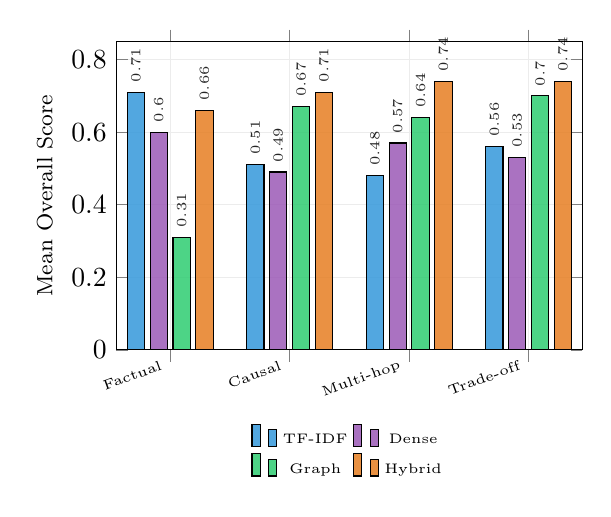
\begin{tikzpicture}
        \begin{axis}[
          ybar,
          bar width=0.22cm,
          width=7.5cm,
          height=5.5cm,
          enlarge x limits=0.15,
          ylabel={\footnotesize Mean Overall Score},
          symbolic x coords={Factual, Causal, Multi-hop, Trade-off},
          xtick=data,
          x tick label style={font=\tiny, rotate=20, anchor=east},
          ymin=0, ymax=0.85,
          legend style={at={(0.5,-0.22)}, anchor=north, legend columns=2,
                         font=\tiny, draw=none},
          every axis plot/.append style={fill opacity=0.85},
          nodes near coords={\pgfmathprintnumber[fixed, precision=2]{\pgfplotspointmeta}},
          every node near coord/.append style={font=\tiny, rotate=90, anchor=west},
          grid=major,
          grid style={gray!15},
        ]
          \addplot[fill=tfidfblue]    coordinates {(Factual,0.710) (Causal,0.510) (Multi-hop,0.480) (Trade-off,0.560)};
          \addplot[fill=densepurple]  coordinates {(Factual,0.600) (Causal,0.490) (Multi-hop,0.570) (Trade-off,0.530)};
          \addplot[fill=graphgreen]   coordinates {(Factual,0.310) (Causal,0.670) (Multi-hop,0.640) (Trade-off,0.700)};
          \addplot[fill=hybridorange] coordinates {(Factual,0.660) (Causal,0.710) (Multi-hop,0.740) (Trade-off,0.740)};
          \legend{TF-IDF, Dense, Graph, Hybrid}
        \end{axis}
      \end{tikzpicture}
    \end{column}
    \begin{column}{0.44\textwidth}
      \textbf{\color{accent}The Story}\\[6pt]
      {\small
        At first, TF-IDF outperformed everything\\
        on overall metrics. Why?\\[4pt]
        Because the initial evaluation was dominated\\
        by \textbf{simple factual} questions --- and\\
        keyword matching is enough for those.\\[8pt]
        When we added \textbf{\color{graphgreen}causal}, \textbf{\color{graphgreen}multi-hop}, and\\
        \textbf{\color{graphgreen}trade-off} questions that require\\
        reasoning about connections...\\[8pt]
      }
      \fcolorbox{graphgreen}{lightgreen}{\parbox{4.5cm}{\centering
        \textbf{\color{graphgreen}The graph effect appeared.}\\[3pt]
        {\small Graph: \textbf{0.670} on causal\\
        vs TF-IDF: 0.510 {\color{accent}(+31\%)}}\\[2pt]
        {\small Hybrid: \textbf{0.740} on multi-hop\\
        vs TF-IDF: 0.480 {\color{accent}(+54\%)}}
      }}
    \end{column}
  \end{columns}
\end{frame}

% ── Slide 15: Thank You ────────────────────────────────────────
{
\setbeamertemplate{footline}{}
\begin{frame}[plain]
  \begin{tikzpicture}[remember picture, overlay]
    \fill[primary] (current page.south west) rectangle (current page.north east);
    \fill[accent, opacity=0.12] ([xshift=4cm, yshift=3cm]current page.south west) circle (6cm);
    \fill[accentblue, opacity=0.15] ([xshift=-2cm, yshift=-1cm]current page.north east) circle (4cm);
    % Thank you
    \node[anchor=center, text=white, font=\Huge\bfseries]
      at ([yshift=2cm]current page.center) {Thank You};
    \draw[accent, line width=1.5pt] ([xshift=-2cm, yshift=0.9cm]current page.center)
      -- ([xshift=2cm, yshift=0.9cm]current page.center);
    % Takeaway
    \node[draw=accent!40, rounded corners=8pt, fill=primary!80, text width=9cm,
          align=center, inner sep=12pt]
      at ([yshift=-0.5cm]current page.center) {
      {\color{white}\normalsize\bfseries Key Takeaway}\\[6pt]
      {\color{white!80}\small
        Traditional search finds \textit{similar text}.\\[2pt]
        GraphRAG finds \textit{connected evidence}.\\[2pt]
        Complex questions need \textit{structured reasoning} ---\\
        and that's exactly what a knowledge graph provides.
      }
    };
    % Author
    \node[anchor=center, text=accent, font=\Large\bfseries]
      at ([yshift=-2.6cm]current page.center) {Jaafar Yeffou};
    \node[anchor=center, text=white!40, font=\small]
      at ([yshift=-3.2cm]current page.center) {GraphRAG for Domain-Specific LLMs --- Generative AI 2025/2026};
  \end{tikzpicture}
\end{frame}
}

\end{document}
